
%(BEGIN_QUESTION)
% Copyright 2006, Tony R. Kuphaldt, released under the Creative Commons Attribution License (v 1.0)
% This means you may do almost anything with this work of mine, so long as you give me proper credit

The following steam boiler is automated with a pneumatic water level transmitter, controller, and control valve.  This system ensures the water level in the steam drum remains approximately constant regardless of changes in steam demand or burner firing rate, and it is called a {\it single-element feedwater control} because it bases the feedwater valve position on a single variable (steam drum level):

$$\includegraphics[width=15.5cm]{i01461x01.eps}$$

The process variable (PV), setpoint (SP), and output signals (manipulated variable, or MV) of the controller are recorded in a table at random time intervals:

% No blank lines allowed between lines of an \halign structure!
% I use comments (%) instead, so that TeX doesn't choke.

$$\vbox{\offinterlineskip
\halign{\strut
\vrule \quad\hfil # \ \hfil & 
\vrule \quad\hfil # \ \hfil & 
\vrule \quad\hfil # \ \hfil \vrule \cr
\noalign{\hrule}
%
% First row
PV & SP & MV \cr
%
(Process Variable) & (Setpoint) & (Output) \cr
%
\noalign{\hrule}
%
% Another row
50\% & 50\% & 50\% \cr
%
\noalign{\hrule}
%
% Another row
48\% & 50\% & 70\% \cr
%
\noalign{\hrule}
%
% Another row
45\% & 50\% & 100\% \cr
%
\noalign{\hrule}
%
% Another row
49\% & 50\% & 60\% \cr
%
\noalign{\hrule}
%
% Another row
52\% & 50\% & 30\% \cr
%
\noalign{\hrule}
%
% Another row
51\% & 50\% & 40\% \cr
%
\noalign{\hrule}
%
% Another row
55\% & 50\% & 0\% \cr
%
\noalign{\hrule}
} % End of \halign 
}$$ % End of \vbox

Based on an examination of the values in this table, is the level controller configured for {\it direct} or {\it reverse} action?

\filbreak

Examining the controller, you notice there is a knob on its side for setting its gain.  This knob is labeled ``Gain / Prop. Band,'' and it has two sets of numbers describing its range of adjustment:

$$\includegraphics[width=15.5cm]{i01461x02.eps}$$

Explain how the two values shown for the knob's setting (Gain = 10 ; Prop. Band = 10\%) relate to the percentages you see in the table.  Particularly, define {\it proportional band} in a way that makes sense looking at the controller's behavior over time.

\vskip 20pt \vbox{\hrule \hbox{\strut \vrule{} {\bf Suggestions for Socratic discussion} \vrule} \hrule}

\begin{itemize}
\item{} Build a computer spreadsheet program to model the behavior of the proportional controller in this scenario.  You will know you are successful when it is able to duplicate the table of values presented in the question (i.e. your spreadsheet will be able to exactly calculate each Output value corresponding to the PV and SP values given in different rows of the table.
\end{itemize}

\underbar{file i01461}
%(END_QUESTION)





%(BEGIN_ANSWER)

This is a {\it reverse-acting} level controller: the output rises when the PV input falls, and vice-versa.

\vskip 10pt

``Proportional band'' is the percentage that the controller input (SP $-$ PV) must deviate in order to swing from 0\% to 100\% on the output.  As you may have noticed, proportional band is the mathematical reciprocal of gain.

%(END_ANSWER)





%(BEGIN_NOTES)



%INDEX% Control, proportional: gain versus proportional band
%INDEX% Control, proportional: proportional band versus gain
%INDEX% Process: steam boiler

%(END_NOTES)


